Les \textit{Level Of Details}, appelés aussi LOD, est une technique qui permet de définir plusieurs niveaux de détails pour un même objet 3D. Cela permet de charger des objets plus ou moins détaillés en fonction de la distance à laquelle ils se trouvent de la caméra. Grâce à cela, il est possible de réduire la charge de travail de l'ordinateur en ne chargeant que le niveau de détail nécessaire pour garder un rendu qui, à l'oeil humain, semble identique à celui d'un rendu contenant tous les objets entièrement détaillés.

Pour calculer le bon niveau de détail à afficher, Cesium utilise le \texttt{bounding volume} ainsi que le \texttt{geometric error} d'une tuile. Le concept est simple, plus un objet occupe une partie importante de la fenêtre de rendu, plus il doit être détaillé. Le \textit{Screen Space Error} ou SSE est une valeur qui permet de déterminer l'imprécision du rendu d'un objet en Pixels. Grâce à elle, il nous est possible de déterminer un seuil SSE auquel Cesium devra changer de LOD. Pour déterminer ce seuil, il nous est possible de définir un \texttt{geometric error} pour chaque tuile. Ce \texttt{geometric error} est une valeur qui permet de déterminer la distance maximale entre la géométrie réelle et la géométrie simplifiée en mètres. Plus cette valeur est grande, plus la géométrie simplifiée sera différent de la géométrie réelle. Avec le \texttt{geometric error}, le \texttt{bounding volume} et la distance entre la caméra et l'objet, il est possible de déterminer le SSE d'une tuile selon la formule suivante :

\begin{equation}
    \centering
    SSE = \frac{geometricError}{distance} \times \frac{screenHeight}{\tan(fovy/2)}
\end{equation}

Où \texttt{screenHeight} est la hauteur de la fenêtre de rendu en pixels et \texttt{fovy} est l'angle de vue de la caméra en radians sur l'axe des y.

Pour plus d'informations, vous pouvez consulter la spécification 3D Tiles \cite{3d-tiles-specification}. Des graphiques tels que celui de la figure \ref{fig:sse} sont disponibles pour mieux comprendre le concept. Le sujet sera abordé à nouveau dans la section \ref{sec:subtrees-intro}.

\begin{figure}[H]
    \centering
    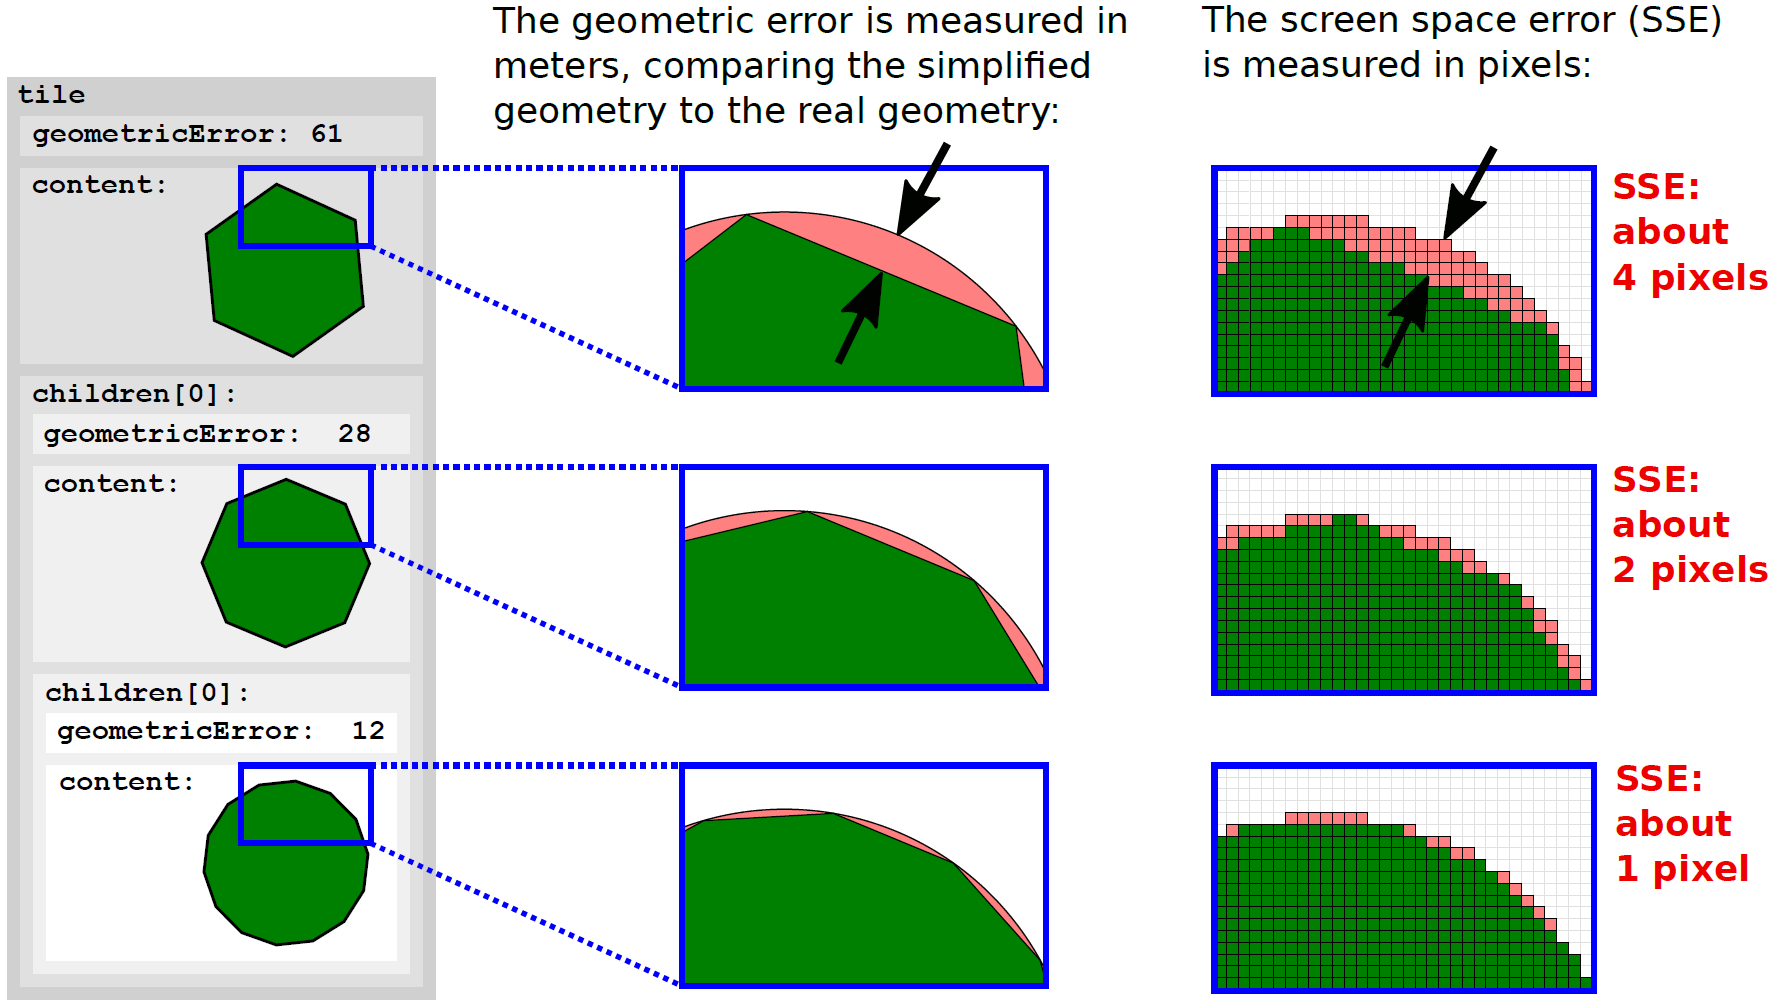
\includegraphics[width=1\textwidth]{assets/figures/sse.png}
    \caption{Calcul du SSE \cite{3d-tiles-specification}}
    \label{fig:sse}
\end{figure}